\begin{figure}[ht]
    \centering
    \begin{subfigure}[t]{0.49\linewidth}
        {\footnotesize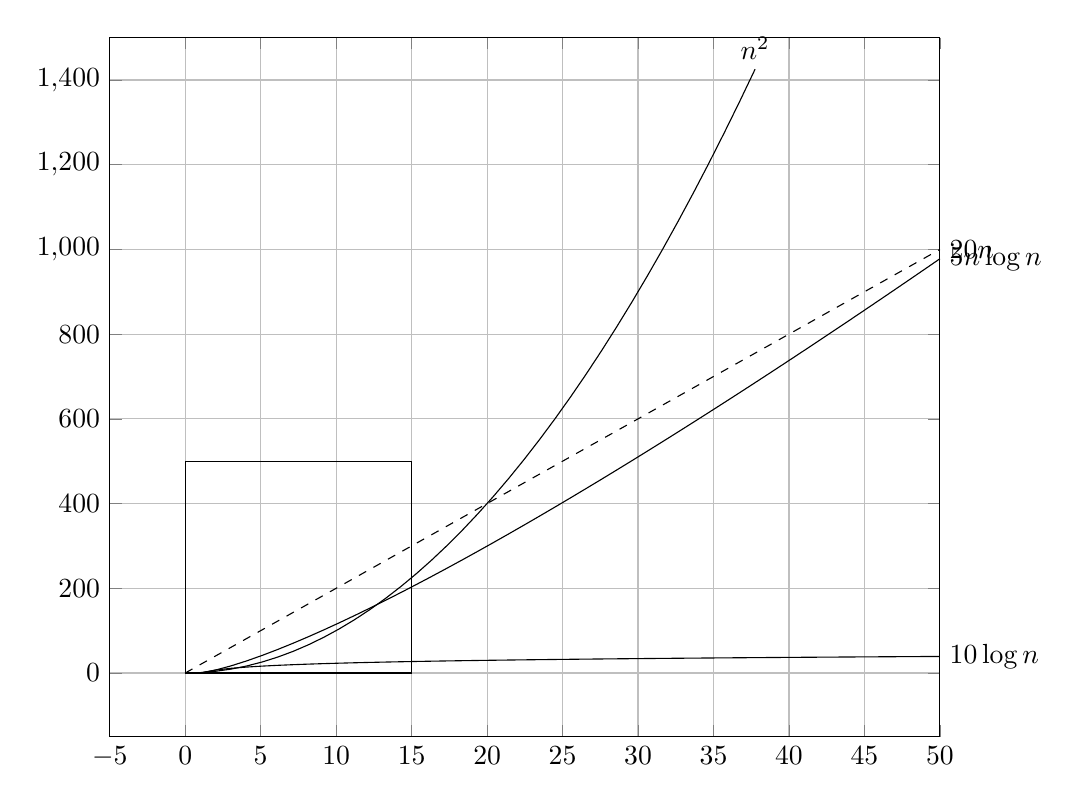
\begin{tikzpicture}
            \begin{axis}[ 
                xlabel={},
                ylabel={},
                width=\textwidth,
                restrict y to domain=0:1500,
                xmax=50,
                ymax=1500,
                samples=50,
                domain=0:50,
                legend pos=north east,
                clip=false,
                grid=both
            ]
                \addplot[dashed]{20 * x} node[right,pos=1] {$20n$};
                \addplot[]{5 * x * ln(x)} node[right,pos=1] {$5n \log n$};
                \addplot[]{10 * ln(x)} node[right,pos=1] {$10\log n$};
                \addplot[]{x^2} node[above,pos=1] {$n^2$};

                \coordinate (origin) at (axis cs:0,0);
                \coordinate (bounding) at (axis cs:15,500);
            \end{axis}

            \draw (origin) rectangle (bounding);
        \end{tikzpicture}}
        \subcaption{Graphen der Wachstumsraten von 4 Funktionen.}
    \end{subfigure}
    \hfill
    \begin{subfigure}[t]{0.49\linewidth}
        {\footnotesize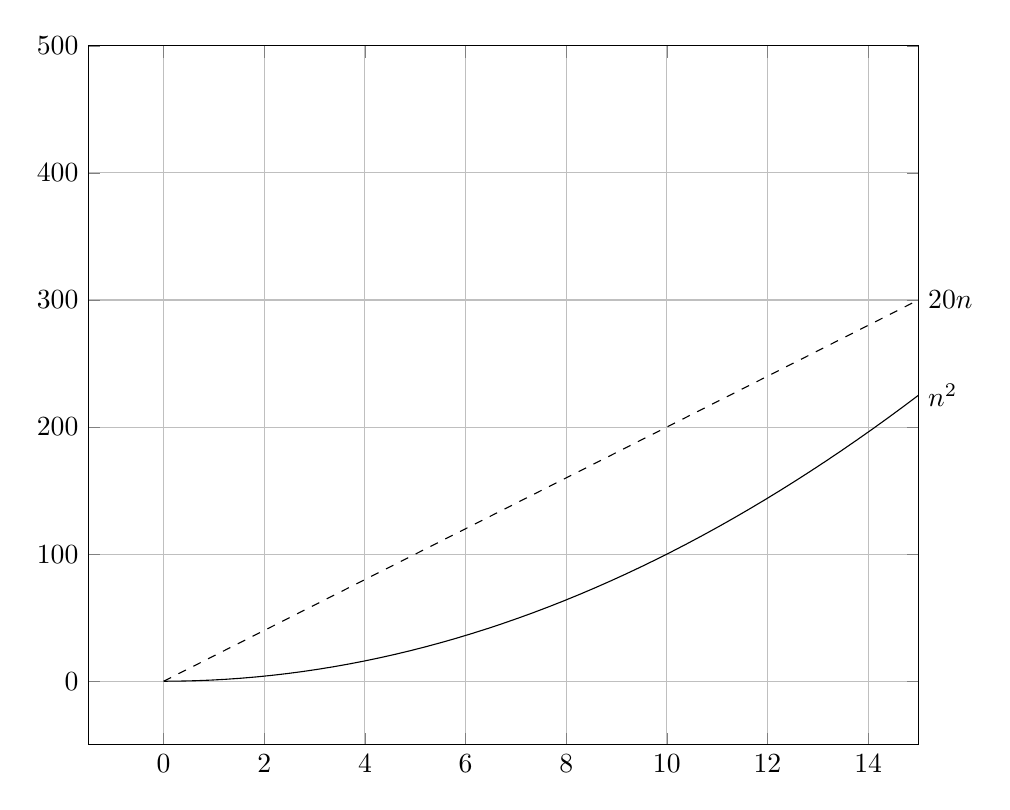
\begin{tikzpicture}
            \begin{axis}[ 
                xlabel={},
                ylabel={},
                width=\textwidth,
                restrict y to domain=0:500,
                grid=both,
                xmax=15,
                ymax=500,
                samples=50,
                domain=0:15,
                legend pos=north east,
                clip=false
            ]
                \addplot[dashed]{20 * x} node[right,pos=1] {$20n$};
                \addplot[]{x^2} node[right,pos=1] {$n^2$};
            \end{axis}
        \end{tikzpicture}}
        \subcaption{Der Inhalt des Rechtecks in (a).}
    \end{subfigure}
    \caption{Zwei Ansichten diverser Graphen der Wachstumsraten einiger Funktionen. Die horizontale Achse repräsentiert im Kontext der Algorithmusanalyse die Eingangsgröße, die vertikale Achse die Anzahl der Operationen (vgl. \cite[57]{sha2011})}
    \label{fig:example-growth-rates-1}
\end{figure}
